\section{Measuring analog voltages}

The core component of the data acquisition is the \href{https://www.raspberrypi.com/documentation/microcontrollers/rp2040.html}{PR2040 Microcontroller} which includes built-in Analog-to-Digital Converters(ADC)\footnote{\href{http://pico-adc.markomo.me/}{This project} is a collection of measurements and analysis in order to document and specify the details of the ADCs of the RP2040 Microcontroller}. These ADCs convert electronic voltages ranging from Ground ($\SI{0}{V}$) to a reference voltage $U_{ref}$ into a digital number defined by the resolution which is depicted in bits. The resolution for all the ADCs in the RP2040 IC is set to 12 bits, meaning that the digital result from an ADC is in between $0$ and $2^{12} = 4096$. Within this conversion the mapping from the analog input voltage to a corresponding digital number should be proportional but has small uncertainties which are defined by the resolution as seen in \cref{fig:ADC-Curve}. This picture also clearly shows that a value acquired by an ADC has an uncertainty of half the voltage to which the least significant bit (LSB) corresponds. This can be calculated as:
\begin{equation*}
	\sigma = \pm{} U_{ref} \cdot \frac{1}{2} \cdot \frac{1}{2^{resolution}} = \pm{} U_{ref} \cdot 2^{-(resolution + 1)}\,.
\end{equation*}

\begin{figure}[htb]
		\centering
		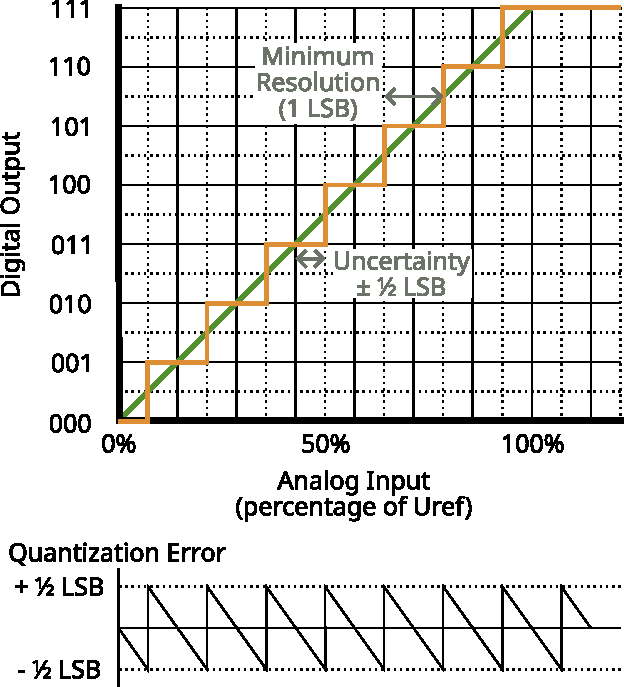
\includegraphics[width=0.6\textwidth]{./fig/ADC-conversion-curve-export.pdf}
		\caption{Conversion from an analog voltage do a digital number with an ADC}
		\label{fig:ADC-Curve}
\end{figure}

In reality there are multiple reasons for small short time fluctuations in the voltage which are greater than the quantization uncertainty of an ADC. Therefore the propper uncertainty of an ADC in an electronic application can be measured with a calibration.
The \href{https://datasheets.raspberrypi.com/rp2040/rp2040-datasheet.pdf}{data sheet} explains that four ADC channels (ADC0 to ADC3) are connected to GPIO Pins and the fifth ADC channel (ADC4) is connected to an internal temperature sensor. Notably the fourth channel ADC3 can be used to measure the VSYS voltage of the Raspberry Pi Pico board.
Each channel is linked to a single Analog-to-Digital Converter (ADC) through an internal switch, allowing the selection of one channel at a time. The shared ADC operates with a maximum sampling rate of 500 kilosamples per second (KSps). This sampling rate can be used for measuring voltages on a single channel at the full sampling speed (simplex). Alternatively, it can simultaneously measure two channels by periodically switching between them, effectively dividing the sampling rate to 250 KSps per channel. The accuracy and the sampling rate are sufficient to use this as the core of a simple oscilloscope which acquires periodically ADC values and streams the data to another device for further processing.

An ADC can only measure voltages between $\SI{0}{V}$ and $U_{ref}$ but we want to build an oscilloscope that can measure positive and negative voltages $\pm{}U_{max}$ within a range of p.ex. $U_{max} > \SI{10}{V}$. It is the task of an analog front-end to map voltages from $-U_{max}$ to $+U_{max}$ into an analog voltage which is suitable for the ADC. Furthermore the range of the input voltage should be selectable and there should be some kind of over-voltage protection on the signal inputs. This allows to measure for higher voltages with less precision or lower voltages with higher precision.

